\documentclass{beamer}
 
\usepackage[utf8]{inputenc}
%\usepackage{fontspec}
%\setmainfont{Linux Libertine O}
%\fontfamily{Computer Modern}\selectfont{Computer Modern Serif}
%\newfontfamily\cmss
 
\usetheme{CambridgeUS} 
%Information to be included in the title page:
\title{Fractais}
\author[Bruno, Mateus]
{Bruno da Silva Esmeraldino  \and Mateus Schroeder da Silva}

\institute{UDESC}
\date{05-2019}
 
 
 
%\logo{
\includegraphics[height=1cm]{images/marca-udesc.png}}
\begin{document}
 
\frame{\titlepage}
 
%\begin{frame}
%\frametitle{AA}
%This is a text in the first frame. This is a text in the first frame. This is a text in the first frame.
%\end{frame}

					
\begin{frame}
\frametitle{Contexto}
	A   primeira   publicação   negando   o   postulado   deve-se   ao   matemático Lobachevski,  em  1826  que,  de  acordo  com  Boyer  (1974,  p.396)  é  chamado  de Copérnico  da  Geometria  de  Lobachevski,  mostrando  com  isso  que  a  geometria euclidiana não era a verdade absoluta que se supunha ser. 
	Hoje  podemos  dizer  que  muitos  problemas  do  cotidiano  e  do  mundo científico não são resolvidos pela geometria euclidiana, mas sim por geometrias não euclidianas,  que  são  aquelas  que  não  satisfazem  um ou  mais  dos  postulados  de Euclides.  Dentro  das  geometrias  não  euclidianas,  entre  outras  podemos  citar,  a Geometria  Hiperbólica;  a  Geometria  Elíptica;  a  Geometria  Projetiva;  a  Topologia;  a Geometriados Fractais. 	Quando nos deparamos com comportamentos na natureza que apresentam formas  tão  irregulares,  como  as  nuvens,  as  montanhas,  os  batimentos  do  coração, as  árvores,  couve-flor,  brócolis  e  entre  outros,  a geometria  euclidiana  por  nós conhecida   se   torna   inadequada,   sendo   necessário   recorrer   a   Geometria   dos Fractais.
\end{frame}

\begin{frame}
\frametitle{Fractais}
	Fractais (do latim fractus, fração, quebrado) são figuras da geometria não-Euclidiana.
 	A geometria fractal é o ramo da matemática que estuda as propriedades e comportamento dos fractais. Descreve muitas situações que não podem ser explicadas facilmente pela geometria clássica, e foram aplicadas em ciência, tecnologia e arte gerada por computador. 
	As raízes conceituais dos fractais remontam a tentativas de medir o tamanho de objetos para os quais as definições tradicionais baseadas na geometria euclidiana falham.
	 Um fractal é um objeto geométrico que pode ser dividido em partes, cada uma das quais semelhante ao objeto original. Diz-se que os fractais têm infinitos detalhes, são geralmente autossimilares e independem de escala. Em muitos casos um fractal pode ser gerado por um padrão repetido, tipicamente um processo recorrente ou iterativo.
\end{frame}
\begin{frame}
	\begin{figure}[htb]
	\centering
    	    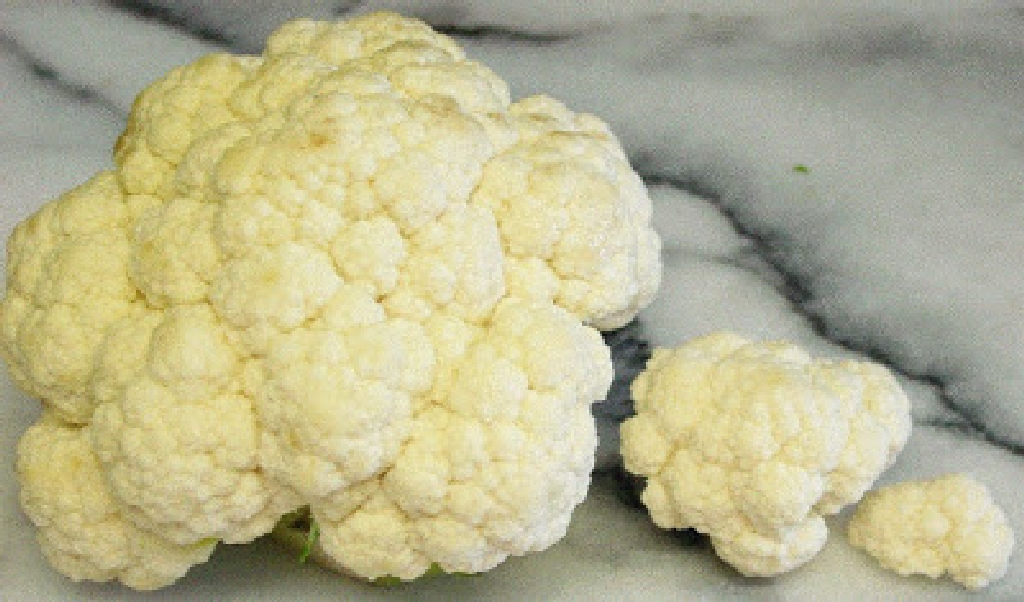
\includegraphics[width=8cm, height=5cm]{images/couve-flor.jpg}
       	        \vspace{0.01em}
       	 %\caption{}
	\end{figure}
\end{frame}

\begin{frame}
\frametitle{Características dos fractais}
Os objetos geométricos fractais podem, infinitamente, ser divididos em partes, sendo que cada uma delas será semelhante à original. Normalmente são autossimilares e não dependem de escalas. Estes fractais podem ser gerados por um padrão repetido. Como exemplo de um fractal, podemos pegar o floco de neve de Koch.
\end{frame}
\begin{frame}
	\begin{figure}[htb]
	\centering
    	    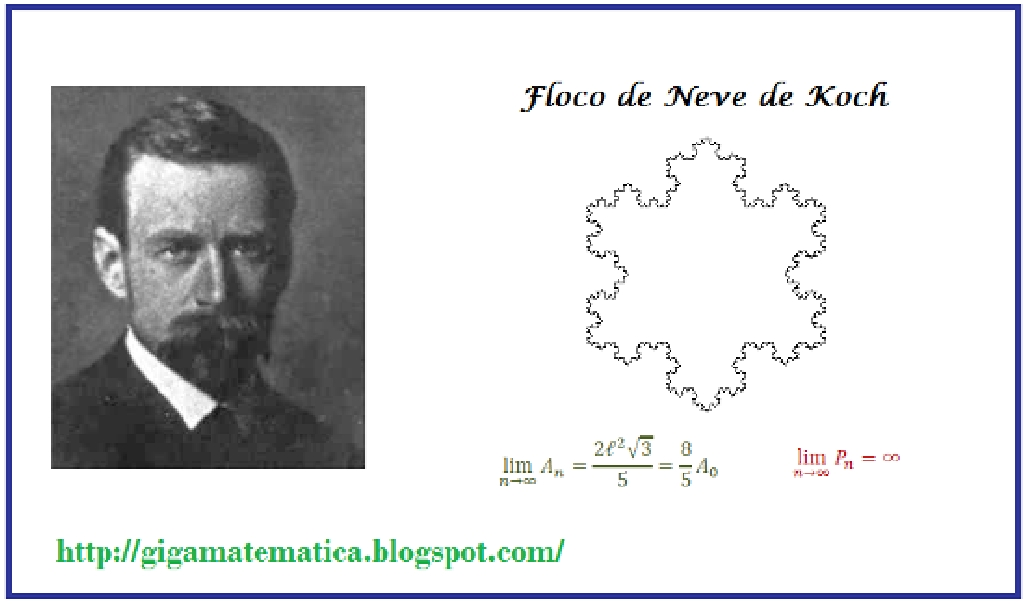
\includegraphics[width=8cm, height=5cm]{images/floco-neve.jpg}
       	        \vspace{0.01em}
       	 %\caption{}
	\end{figure}
\end{frame}
\begin{frame}
\frametitle{Geometria de fractais determinísticos}
Neste caso, estamos falando de subconjuntos que são gerados por transformações geométricas simples que acontecem do objeto nele mesmo, ou seja, o objeto é formado por ele mesmo em formas reduzidas.
\end{frame}
\begin{frame}
	\begin{figure}[htb]
	\centering
    	    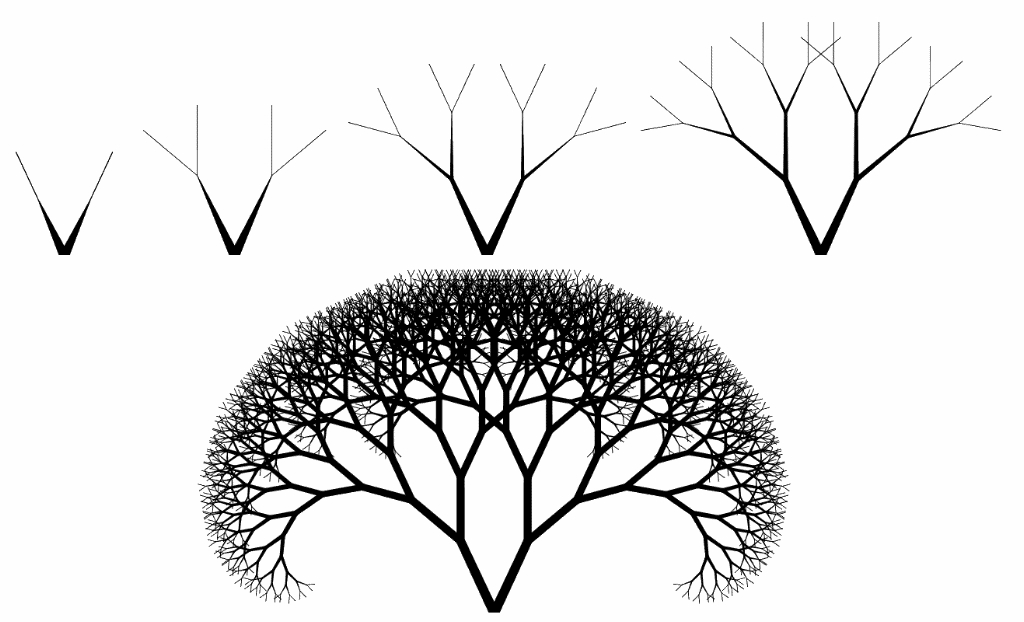
\includegraphics[width=8cm, height=5cm]{images/arvore.jpg}
       	        \vspace{0.01em}
       	 %\caption{}
	\end{figure}
\end{frame}
\begin{frame}
\frametitle{A história}
Alguns cientistas, em seus trabalhos, entre os anos de 1857 e 1913, desenvolveram o conhecimento de alguns objetos que até então eram catalogados como demônios, supondo que não teriam grandes valores científicos. Weiertrass, no ano de 1872, encontrou uma função contínua em todo o seu domínio, chamado atualmente de fractal. Koch, no entanto, não se viu satisfeito com essa definição abstrata demais, dando uma definição mais geométrica de uma função similar, que é o floco de neve de Koch. O desenho desse floco de neve é resultado da infinita adição de triângulos que fazem com que o perímetro cresça aproximando-se do infinito.
\end{frame}
\begin{frame}
Muitos outros trabalhos estiveram relacionados à essa ideia do fractal, mas somente nos anos 60, quando a computação surgiu, seu desenvolvimento se deu. Mandelbrot, o criador do termo fractal e responsável pela descoberta do conjunto de Mandelbrot, um dos fractais mais conhecidos, foi um dos pioneiros a fazer uso dessa técnica para desenvolver seus estudos.
Esse foi o primeiro homem a descrever o mundo da forma como ele é. Antes do polonês Benoit Mandelbrot, quase toda a geometria que conhecíamos era aquela fundada pelo grego Euclides por volta de 300 a.C., a das linhas, pontos, esferas, cones… Enfim, tudo aquilo que as escolas ensinam. O problema é que essas formas euclidianas são artificiais. Funcionam para traduzir a harmonia da matemática, mas não estão na natureza. Não existem montanhas em forma de cone, nuvens triangulares, animais cúbicos. 
\end{frame}
\begin{frame}
\frametitle{Aplicações}
\end{frame}
\begin{frame}
\frametitle{Medicina}
A estrutura do pulmão e as ramificações dos neurônios remetem a essas figuras. Entre outros benefícios, a compreensão do desenvolvimento dos fractais pode ajudar a prever a evolução de doenças como o câncer, facilitando diagnósticos precoces.
\end{frame}
\begin{frame}
	\begin{figure}[htb]
	\centering
    	    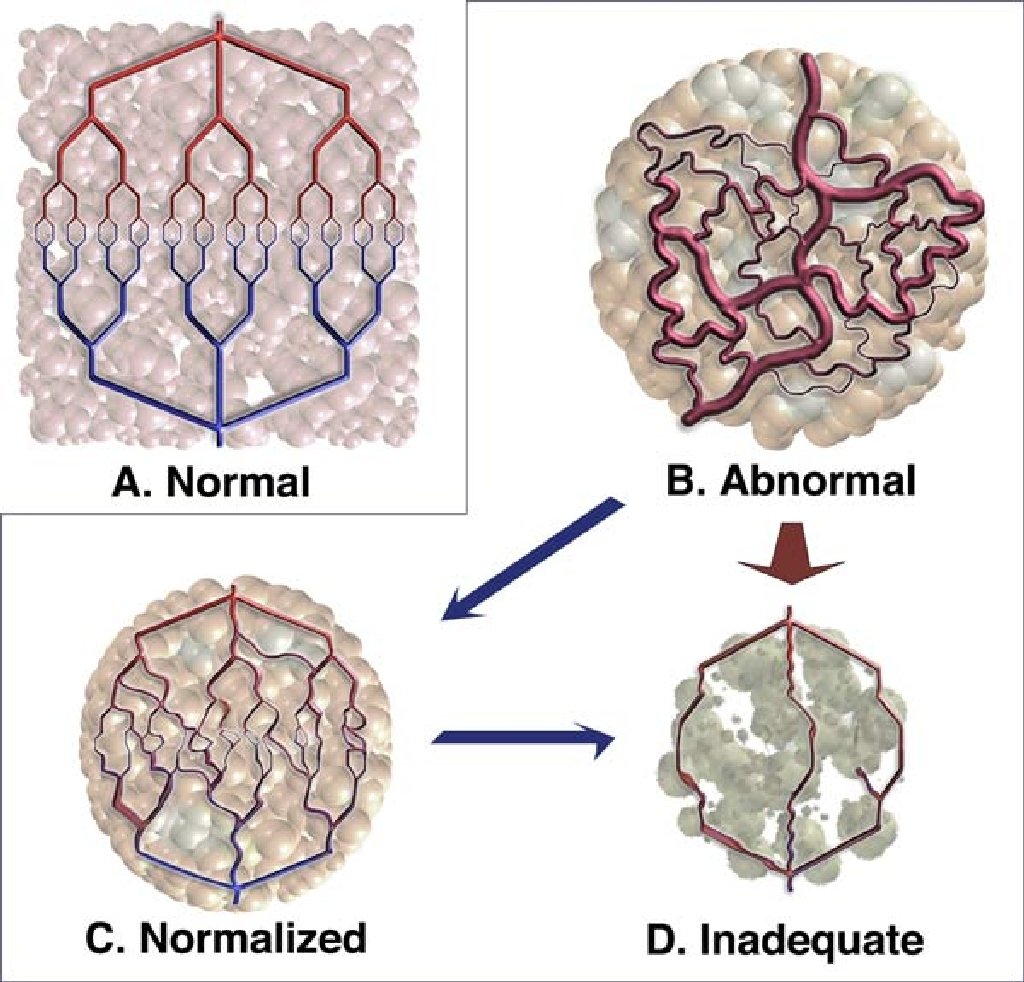
\includegraphics[width=8cm, height=5cm]{images/medicina.jpg}
       	        \vspace{0.01em}
       	 %\caption{}
	\end{figure}
\end{frame}
\begin{frame}
\frametitle{Computação gráfica}
Alguns tipos têm sido utilizados como base de animações digitais. Eles ajudam a criar texturas, simular vegetação ou construir paisagens complexas. Apollo 13 (1995) e Titanic (1997) são alguns filmes que aplicaram esse recurso.
\end{frame}
\begin{frame}
	\begin{figure}[htb]
	\centering
    	    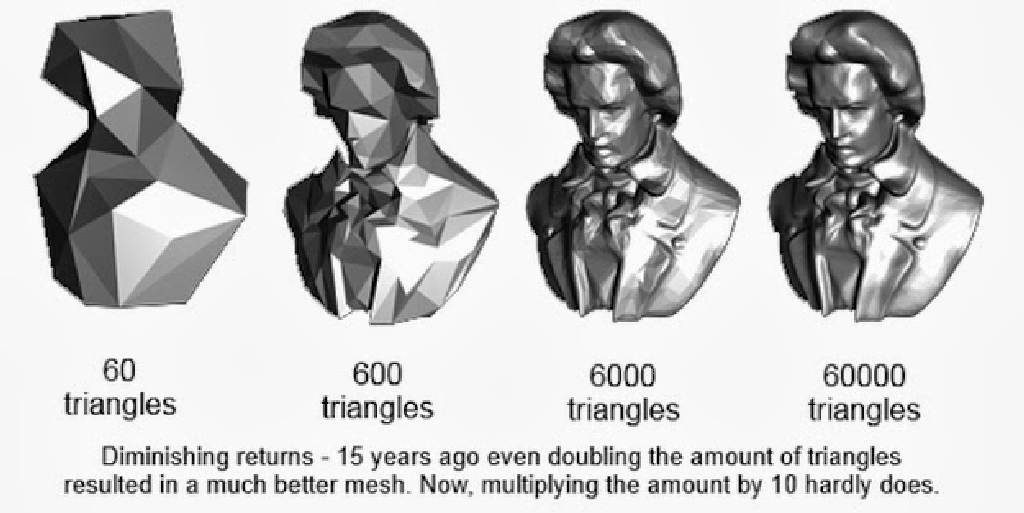
\includegraphics[width=8cm, height=5cm]{images/comp1.jpg}
       	        \vspace{0.01em}
       	 %\caption{}
	\end{figure}
\end{frame}
\begin{frame}
	\begin{figure}[htb]
	\centering
    	    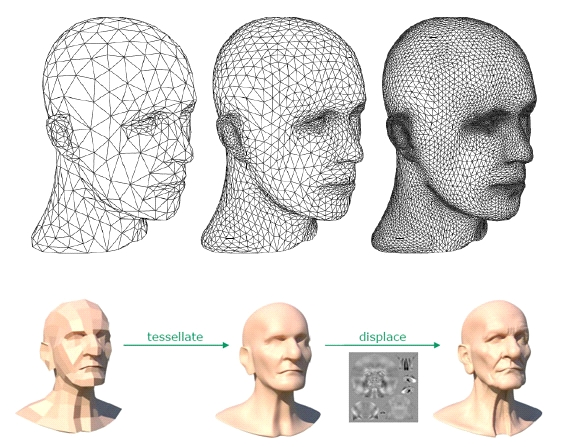
\includegraphics[width=8cm, height=5cm]{images/comp2.jpg}
       	        \vspace{0.01em}
       	 %\caption{}
	\end{figure}
\end{frame}
\begin{frame}
\frametitle{Geografia}
Os dobramentos das camadas de rocha que formam o solo são criados por dobramentos ainda menores, como um fractal. Ao se definir, por computador, esses padrões, pode-se estudar a instabilidade dos solos e prevenir catástrofes como a da região serrana do Rio de Janeiro.
\end{frame}
\begin{frame}
	\begin{figure}[htb]
	\centering
    	    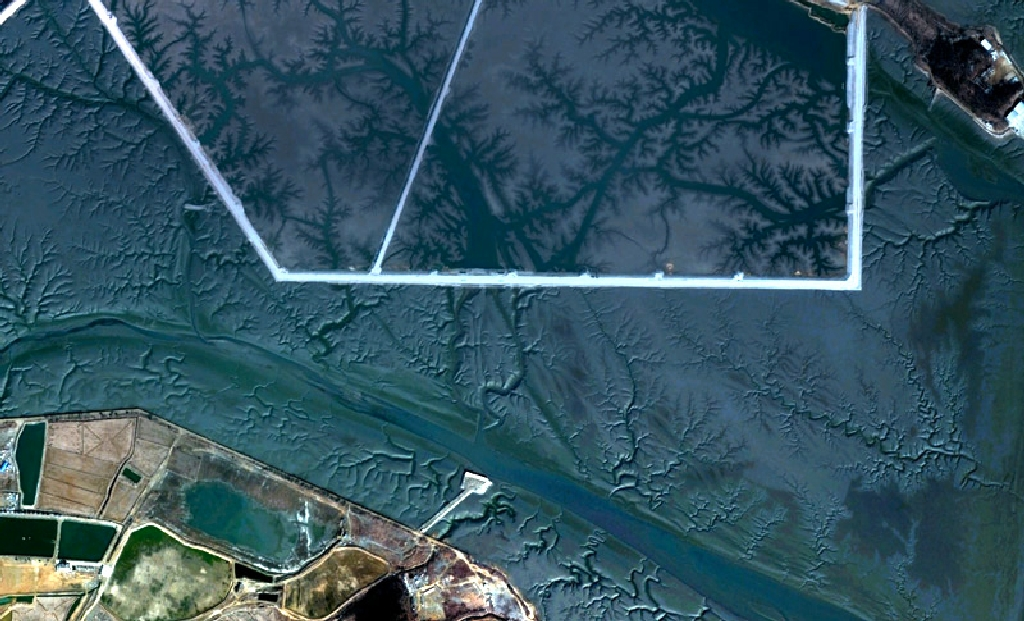
\includegraphics[width=8cm, height=5cm]{images/geo1.jpg}
       	        \vspace{0.01em}
       	 %\caption{}
	\end{figure}
\end{frame}
\begin{frame}
\frametitle{Economia}
O conceito de fractal é usado no entendimento do comportamento da Bolsa de Valores. A variação do valor da ação em um dia de pregão é similar à variação de uma semana, um mês, um ano ou uma década. Com isso, é possível fazer estatísticas mais precisas.
\end{frame}
\begin{frame}
	\begin{figure}[htb]
	\centering
    	    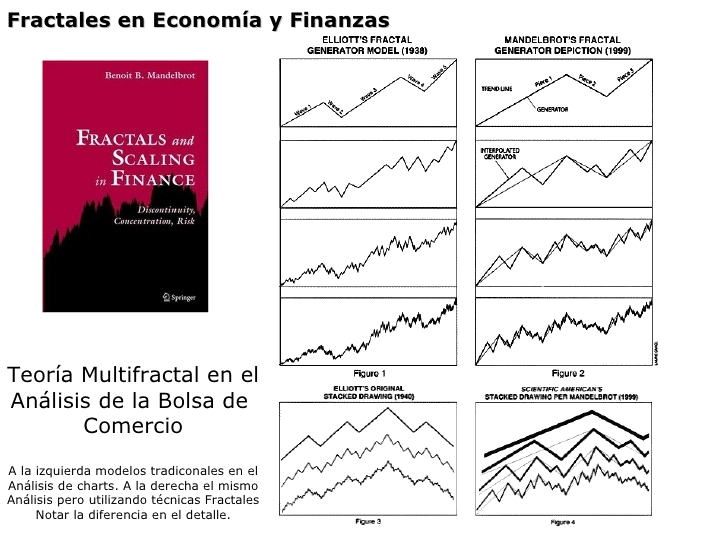
\includegraphics[width=8cm, height=5cm]{images/eco1.jpg}
       	        \vspace{0.01em}
       	 %\caption{}
	\end{figure}
\end{frame}
\begin{frame}
\frametitle{Arte}
Arte fractal é a criada utilizando-se funções matemáticas chamadas fractais e transformando os resultados dos cálculos em imagens, animações, música ou outro tipo de mídia. Imagens fractais são os gráficos resultante dos cálculos, e animações são seqüências desses gráficos. Música fractal transforma os resultados do cálculo em sons. Geralmente, mas não exclusivamente, utilizam-se computadores para processá-los, devido à complexidade da matemática envolvida. 
\end{frame}
\begin{frame}
	\begin{figure}[htb]
	\centering
    	    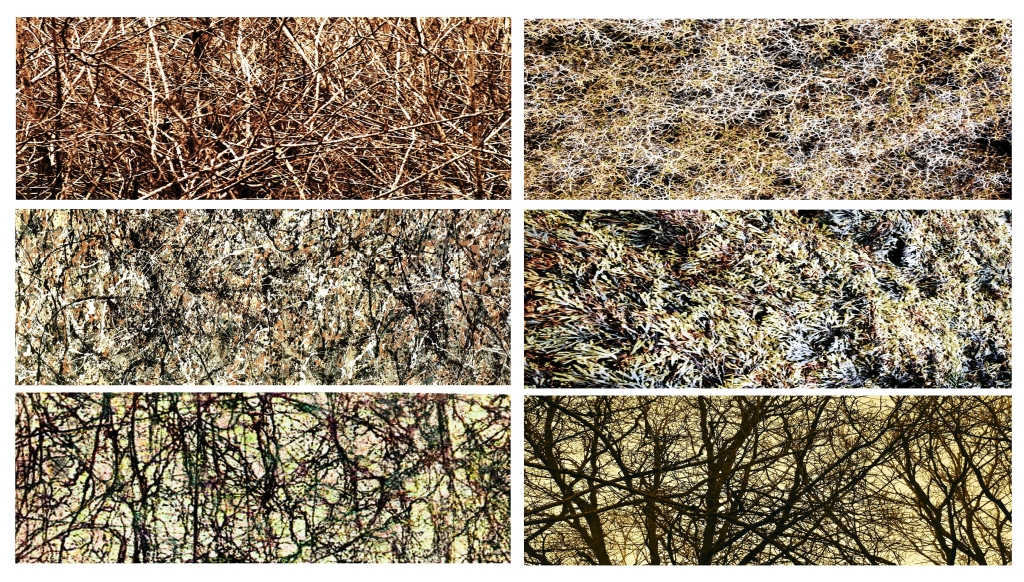
\includegraphics[width=8cm, height=5cm]{images/art1.jpg}
       	        \vspace{0.01em}
       	 %\caption{}
	\end{figure}
\end{frame}
\begin{frame}
	\begin{figure}[htb]
	\centering
    	    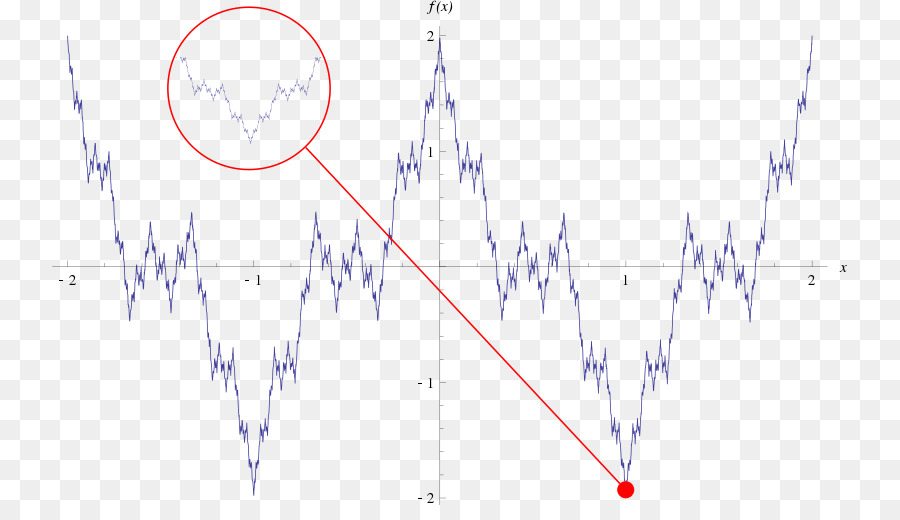
\includegraphics[width=8cm, height=5cm]{images/strass.jpg}
       	        \vspace{0.01em}
       	 \caption{Função de Weiertrass}
	\end{figure}
    Exemplo de função patológica: contínua em todos os pontos da reta mas em nenhum ponto derivável. Weiertrass (1815-1897).
\end{frame}
\begin{frame}
	\begin{figure}[htb]
	\centering
    	    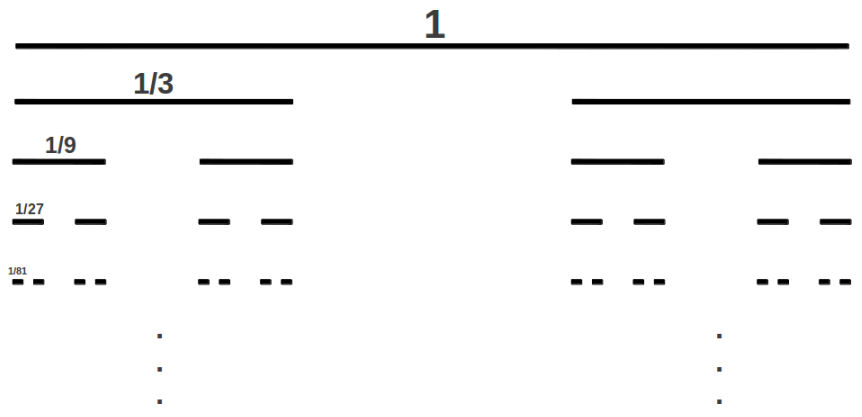
\includegraphics[width=8cm, height=5cm]{images/cs1.jpg}
       	        \vspace{0.01em}
            \caption{Conjunto de Cantor}
	\end{figure}
\end{frame}
\begin{frame}
	\begin{figure}[htb]
	\centering
    	    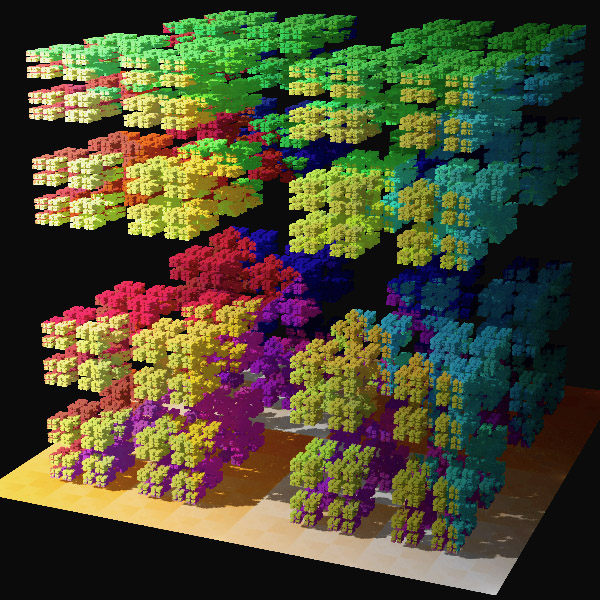
\includegraphics[width=8cm, height=5cm]{images/cs2.jpg}
       	        \vspace{0.01em}
	\end{figure}
\end{frame}
\begin{frame}
	\begin{figure}[htb]
	\centering
    	    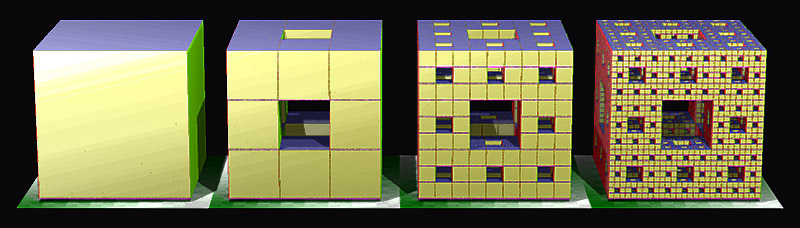
\includegraphics[width=8cm, height=3cm]{images/sponge.jpg}
       	        \vspace{0.01em}
       	 \caption{Esponja de Menger}
	\end{figure}
\end{frame}
\begin{frame}
    \frametitle{Dimensões}
    \centering
        De Hausdorff \\
        Topológica
\end{frame}
\begin{frame}
	\begin{figure}[htb]
	\centering
    	    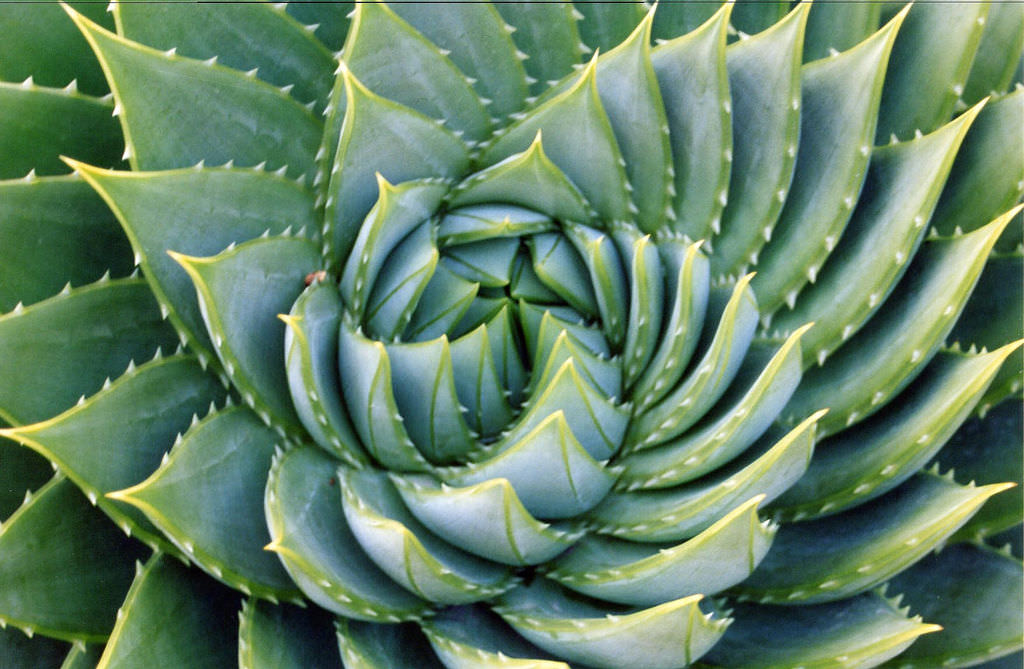
\includegraphics[width=8cm, height=5cm]{images/nat1.jpg}
       	        \vspace{0.01em}
	\end{figure}
\end{frame}
\begin{frame}
	\begin{figure}[htb]
	\centering
    	    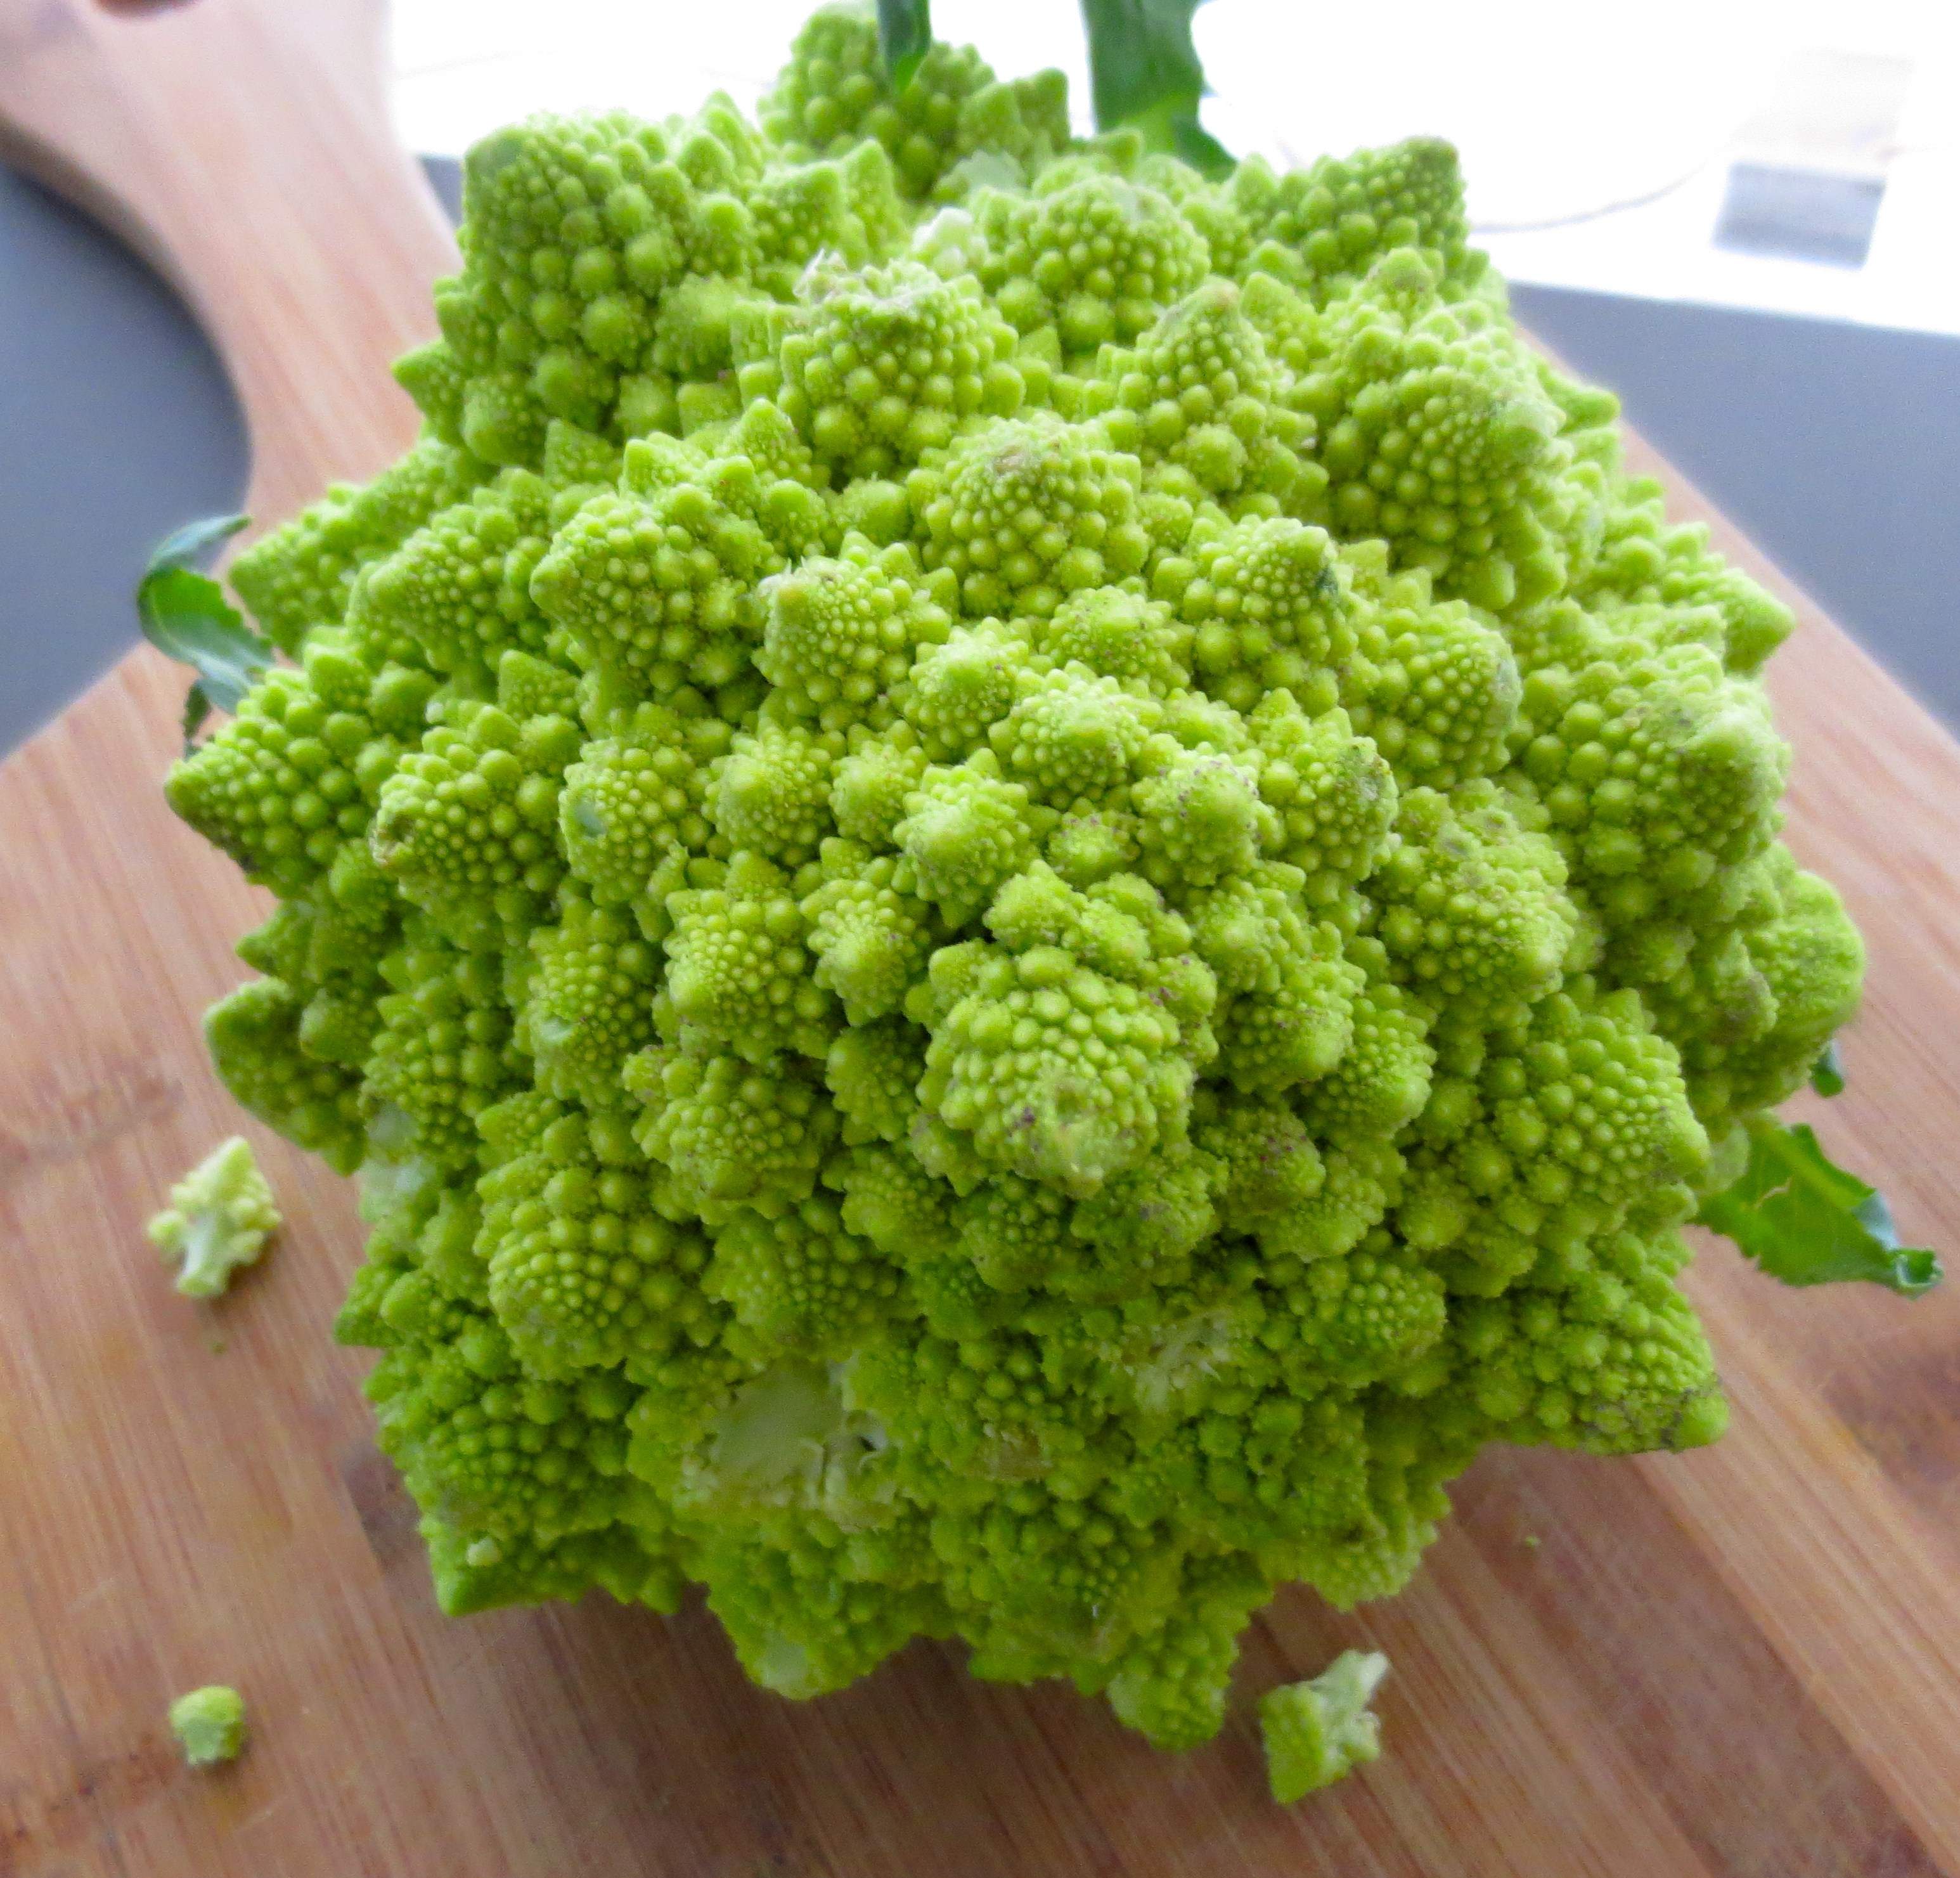
\includegraphics[width=7cm, height=4cm]{images/broc.jpg}
       	        \vspace{0.01em}
                \caption{Romanesco Broccoli}
	\end{figure}
\end{frame}

\begin{frame}
    Artistas importantes: \\
    Desmond Paul Henry \\
    Hamid Naderi Yeganeh \\
    Bruno Degazio

\end{frame}
\begin{frame}
	\begin{figure}[htb]
	\centering
    	    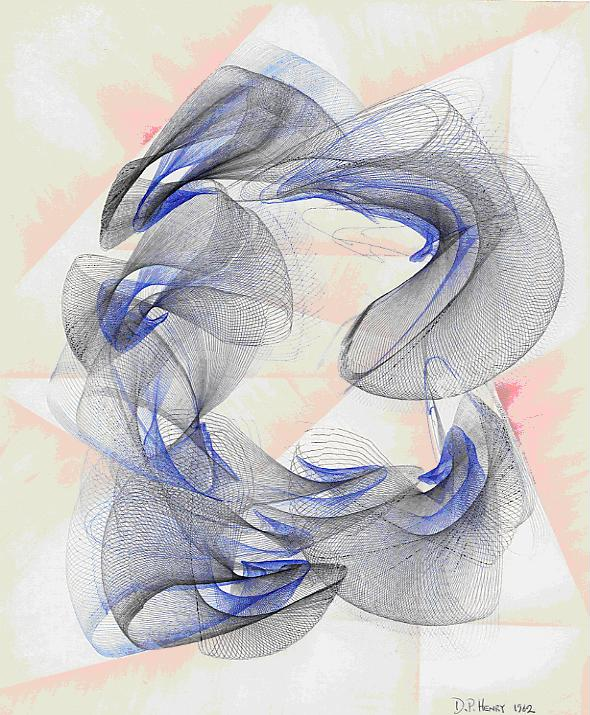
\includegraphics[width=7cm, height=4cm]{images/dr1.jpg}
       	        \vspace{0.01em}
                \caption{Gerado por máquina, Henry}
	\end{figure}
\end{frame}
\begin{frame}
	\begin{figure}[htb]
	\centering
    	    
\includegraphics[width=7cm, height=4cm]{images/hamid1.jpg}
       	        \vspace{0.01em}
                \caption{Heart, Hamid}
	\end{figure}
\end{frame}
%\begin{frame}
%	\begin{figure}[htb]
%	\centering
%    	    \includegraphics[width=8cm, height=5cm]{images/.jpg}
%       	        \vspace{0.01em}
%       	 %\caption{}
%	\end{figure}
%\end{frame}
\end{document}
